\documentclass[11pt]{article}

% ── packages ──────────────────────────────────────────────────────────────────
\usepackage[margin=1in]{geometry}
\usepackage{amsmath,amssymb,amsthm}
\usepackage{booktabs}
\usepackage{graphicx}
\usepackage{hyperref}
\usepackage{natbib}
\usepackage{microtype}
\usepackage{listings}
\usepackage{xcolor}
\usepackage{bm}

% ── code style ────────────────────────────────────────────────────────────────
\definecolor{codegray}{rgb}{0.95,0.95,0.95}
\definecolor{codeblue}{rgb}{0.0,0.3,0.7}
\lstset{
  backgroundcolor=\color{codegray},
  basicstyle=\ttfamily\small,
  keywordstyle=\color{codeblue}\bfseries,
  commentstyle=\color{gray},
  frame=single,
  framerule=0.4pt,
  breaklines=true,
  language=Python,
  showstringspaces=false,
}

% ── theorem environments ──────────────────────────────────────────────────────
\newtheorem{theorem}{Theorem}
\newtheorem{proposition}{Proposition}
\newtheorem{lemma}{Lemma}
\newtheorem{definition}{Definition}
\newtheorem{remark}{Remark}

% ── title ─────────────────────────────────────────────────────────────────────
\title{One-Pass Exact Hessians via Hypercomplex Perturbation:\\
       A Vectorized Implementation with Implicit Layer Applications}
\author{Zetta Byte}
\date{April 2, 2026}

\begin{document}
\maketitle

% ── abstract ──────────────────────────────────────────────────────────────────
\begin{abstract}
Second-order information is central to optimization, sensitivity analysis, and the
study of implicit models, but computing full Hessians remains prohibitively expensive
for all but the smallest systems. This work introduces a vectorized hypercomplex
perturbation method that recovers exact first- and second-order derivatives of
scalar-valued functions in a single forward evaluation. By augmenting each input with
a pair of commuting infinitesimal units, the method embeds the full Taylor expansion
into an extended algebra whose coefficient channels isolate the gradient and Hessian
without approximation. The resulting implementation achieves near-gradient cost for
dimensions up to $n \sim 100$, providing exact curvature in a regime where diagonal
approximations offer limited value.

We present a NumPy-based reference implementation with complete reproducibility,
a validated test suite, and empirical benchmarks across polynomial, transcendental,
and implicit functions. For fixed-point models, the method recovers the
implicit-function-theorem Hessian directly, avoiding the iteration-dependent curvature
produced by unrolled differentiation. The approach is not intended for deep networks,
where the Hessian is too large to represent explicitly, but instead fills the
exact/moderate-$n$ region of the cost--accuracy landscape. The method provides a
practical primitive for scientific computing, differentiable physics, and
curvature-aware optimization, and establishes a foundation for JAX/XLA backends and
higher-order extensions.
\end{abstract}

% ── 1. introduction ───────────────────────────────────────────────────────────
\section{Introduction}

Second-order information plays a central role in optimization, sensitivity analysis,
and the study of implicit models. Curvature governs stability, trust-region behavior,
and the geometry of parameter updates, yet computing full Hessians remains expensive
for all but the smallest systems. Reverse-mode algorithmic differentiation (AD)
requires $O(n)$ reverse passes for an $n$-dimensional input, while forward-over-reverse
strategies incur implementation-dependent constants. Diagonal approximations scale to
deep networks but discard off-diagonal structure by design. As a result, exact
second-order methods are often treated as impractical outside of toy problems.

This work revisits the problem from a different angle. Instead of extending AD or
approximating curvature, we modify the representation of the input itself. By
augmenting each coordinate with a pair of commuting infinitesimal units, the full
first- and second-order Taylor expansion of a scalar function $f:\mathbb{R}^n \to
\mathbb{R}$ is embedded directly into an extended algebra. A single forward evaluation
of $f$ in this algebra recovers the gradient and Hessian exactly, with no reverse pass
and no approximation. The cost is dominated by arithmetic in a coefficient vector of
length $1 + 3n + \frac{n(n-1)}{2}$, making the method practical for moderate
dimensions ($n \sim 2$ to $100$) where exact curvature is valuable and diagonal
approximations offer limited benefit.

We present a vectorized implementation of this hypercomplex perturbation method,
together with a complete test suite, reproducible benchmarks, and applications to
implicit fixed-point models. For implicit systems $z^* = f(z^*, \theta)$, the method
recovers the implicit-function-theorem Hessian directly by perturbing the converged
fixed point, avoiding the iteration-dependent curvature produced by unrolled
differentiation. Empirically, the vectorized core achieves near-gradient wall-clock
cost while returning the full Hessian exactly across a range of polynomial,
transcendental, and implicit functions.

The goal of this work is not to replace scalable diagonal approximations in deep
learning, where the Hessian is too large to represent explicitly. Rather, it fills the
exact/moderate-$n$ region of the cost--accuracy landscape that remains underserved:
scientific computing, differentiable physics, implicit layers, and small neural
modules where full curvature is both meaningful and computationally accessible. The
method provides a simple, algebraic, and reproducible primitive for exact second-order
computation, and establishes a foundation for JAX/XLA backends and higher-order
extensions.

% ── 2. background ─────────────────────────────────────────────────────────────
\section{Background}

\subsection{The Complex-Step Method}

The complex-step method \citep{lyness1967,squire1998} perturbs a real function into
the complex plane to obtain machine-precision first derivatives without cancellation
error. For $f:\mathbb{R} \to \mathbb{R}$ and small $h$:
\[
  f'(x) = \frac{\operatorname{Im}[f(x + ih)]}{h} + O(h^2).
\]
The imaginary part extracts the derivative exactly because complex arithmetic
separates real and imaginary components without subtraction. This avoids the
cancellation error that limits finite differences at small $h$.

The approach does not extend to second derivatives without additional structure:
$\operatorname{Im}[f(x+ih)] / h$ gives the gradient, but the Hessian requires a
second perturbation direction that does not interact with the first.

\subsection{Dual Numbers and Automatic Differentiation}

Dual numbers augment the real line with a nilpotent unit $\varepsilon$ satisfying
$\varepsilon^2 = 0$. For $x = a + b\varepsilon$:
\[
  f(a + b\varepsilon) = f(a) + b\,f'(a)\,\varepsilon.
\]
This gives exact first derivatives in one forward pass and is the basis of
forward-mode automatic differentiation. The nilpotent condition truncates the Taylor
series exactly at first order.

Combining both units gives the \emph{hyper-dual} numbers
\citep{griewank2008}: augment with $\varepsilon_1, \varepsilon_2$ satisfying
$\varepsilon_i^2 = 0$. Then:
\[
  f(a + \varepsilon_1 + \varepsilon_2)
  = f(a) + f'(a)(\varepsilon_1 + \varepsilon_2) + f''(a)\,\varepsilon_1\varepsilon_2.
\]
The cross-term $\varepsilon_1\varepsilon_2$ isolates $f''(a)$ exactly for univariate
functions.

\subsection{Extending to Multiple Dimensions}

For $f:\mathbb{R}^n \to \mathbb{R}$, the Hessian has $n^2$ entries. We need $n$
imaginary directions (one per input) and $n$ nilpotent directions. The hypercomplex
algebra used in this work assigns to each coordinate $x_j$ a pair of units:
\[
  X_j = x_j + \alpha\,i_j + \beta\,\varepsilon_j,
\]
where $i_j^2 = -1$ (imaginary) and $\varepsilon_j^2 = 0$ (nilpotent), and all units
commute. The imaginary channel $i_j$ carries first-order information; the mixed
channel $i_j\varepsilon_k$ carries the $(j,k)$ Hessian entry.

% ── 3. algebra ────────────────────────────────────────────────────────────────
\section{The Hypercomplex Algebra}

\subsection{Coefficient Layout}

A hypercomplex number with $n$ input dimensions is represented as a vector of
$1 + 3n + \tfrac{n(n-1)}{2}$ coefficients:

\begin{center}
\begin{tabular}{lll}
\toprule
Index range & Basis element & Content \\
\midrule
$[0]$               & $1$             & real part \\
$[1, \ldots, n]$    & $i_j$           & gradient channels \\
$[n+1, \ldots, 2n]$ & $\varepsilon_j$ & nilpotent channels \\
$[2n+1, \ldots, 3n]$& $i_j\varepsilon_j$ & diagonal Hessian \\
$[3n+1, \ldots]$    & $i_j\varepsilon_k,\; j < k$ & off-diagonal Hessian \\
\bottomrule
\end{tabular}
\end{center}

\subsection{Multiplication Rules}

The algebra is defined by:
\[
  i_j^2 = -1, \quad \varepsilon_j^2 = 0, \quad \varepsilon_j\varepsilon_k = 0
  \;\text{for}\; j \neq k, \quad [i_j, \varepsilon_k] = 0 \;\text{(commutative)}.
\]
Products at higher order truncate because $\varepsilon_j^2 = 0$ kills any term
involving a repeated nilpotent unit. The key multiplication result is:
\[
  i_j \cdot \varepsilon_k =
  \begin{cases} i_j\varepsilon_j & j = k \\ i_j\varepsilon_k & j < k \end{cases}
\]
which places Hessian information in distinct basis elements.

\subsection{Extraction}

Given the hypercomplex result $F = f(X_0, \ldots, X_{n-1})$, the gradient and Hessian
are extracted as:
\begin{align}
  \frac{\partial f}{\partial x_j} &= \frac{[F]_{i_j}}{\alpha}, \\
  \frac{\partial^2 f}{\partial x_j \partial x_k} &=
    \frac{[F]_{i_j\varepsilon_k}}{\alpha\beta} \quad (j \leq k).
\end{align}
The real part $[F]_1 = f(x)$ gives the function value simultaneously.

\subsection{Correctness}

\begin{proposition}
For any twice-differentiable scalar function $f:\mathbb{R}^n \to \mathbb{R}$,
evaluation at the hypercomplex seed $X_j = x_j + \alpha i_j + \beta\varepsilon_j$
recovers $\nabla f(x)$ and $\nabla^2 f(x)$ exactly from the coefficient channels,
with no truncation error and no dependence on $\alpha$ or $\beta$ (provided both
are nonzero).
\end{proposition}

\begin{proof}
By the multivariate Taylor expansion and the multiplication rules, the
$i_j\varepsilon_k$ coefficient of $f(X)$ equals $\alpha\beta \cdot \partial^2 f /
\partial x_j \partial x_k$ exactly. The nilpotent condition $\varepsilon_j^2 = 0$
truncates the Taylor series at second order, and the commutativity of all units
ensures the mixed partial is recovered without ordering ambiguity.
\end{proof}

% ── 4. implementation ─────────────────────────────────────────────────────────
\section{Implementation}

\subsection{Prototype vs Vectorized Core}

The v0.1.0 implementation served as an algebraically correct prototype.
Its \texttt{\_\_mul\_\_} method accumulated the mixed-term contributions
$\langle i_j \varepsilon_k \rangle$ using a double Python loop:

\begin{lstlisting}
# v0.1.0 -- O(n^3) per multiply
for j in range(n):
    for k in range(n):
        contrib = (a[idx_i(j)] * b[idx_eps(k)]
                   + b[idx_i(j)] * a[idx_eps(k)])
        if j == k:
            out[idx_diag_mix(j)] += contrib
        elif j < k:
            out[idx_mix(j, k)] += contrib   # idx_mix itself is O(n^2)
\end{lstlisting}

The index helper \texttt{idx\_mix(j,k)} contained a further Python double loop
to locate the off-diagonal coefficient, making the effective cost
$O(n^3)$ per multiplication in Python interpreter overhead alone.

\subsection{v0.2.0 Vectorization}

The v0.2.0 core eliminates every Python loop from the hot path.

\paragraph{Index precomputation.}
At construction time (cached by $n$ via \texttt{functools.lru\_cache}), we build:
\begin{lstlisting}
js, ks = np.triu_indices(n, k=1)   # upper-triangle pairs, lex order
\end{lstlisting}
These integer arrays of length $n(n-1)/2$ are computed once and reused
for every multiply.

\paragraph{Multiplication via outer product and gather.}
The entire mixed-term accumulation reduces to:
\begin{lstlisting}
P = np.outer(a_i, b_eps) + np.outer(b_i, a_eps)  # shape (n, n)
out[sl_diag] += np.diag(P)       # diagonal: j == k
out[sl_off]  += P[js, ks]        # off-diagonal: j < k, lex order
\end{lstlisting}
Two \texttt{np.outer} calls (BLAS \texttt{dger}), one \texttt{np.diag}, and one
fancy-index gather replace $O(n^2)$ Python iterations.

\paragraph{Vectorized unary operations.}
All transcendental functions follow the chain-rule pattern
$f(a + \delta) \approx f(a) + f'(a)\delta + \tfrac{1}{2}f''(a)\delta^2$.
A shared helper \texttt{\_apply\_scalar\_func($f_0$, $f_1$, $f_2$)} applies this
in array slices:
\begin{lstlisting}
out[sl_diag] = f1 * c[sl_diag] + f2 * c_i * c_eps
out[sl_off]  = f1 * c[sl_off]  + f2*(c_i[js]*c_eps[ks]
                                      + c_i[ks]*c_eps[js])
\end{lstlisting}
\texttt{exp}, \texttt{tanh}, \texttt{sin}, \texttt{cos}, \texttt{sigmoid},
\texttt{sqrt}, and \texttt{log} all call this helper. No Python loops remain in
the hot path.

\subsection{Measured Speedup}

Table~\ref{tab:speedup} shows the per-\texttt{\_\_mul\_\_} speedup on a NumPy
backend (single call, excluding Python dispatch overhead).

\begin{table}[h]
\centering
\caption{Single \texttt{\_\_mul\_\_} call timing: v0.1.0 vs v0.2.0 (NumPy backend).}
\label{tab:speedup}
\begin{tabular}{rrrr}
\toprule
$n$ & v0.1.0 ($\mu$s) & v0.2.0 ($\mu$s) & Speedup \\
\midrule
  4 &       18        &       13        &  1.4$\times$ \\
  8 &       55        &       13        &  4$\times$   \\
 16 &      331        &       14        &  23$\times$  \\
 32 &    3,262        &       30        & 108$\times$  \\
 64 &   57,051        &      188        & 303$\times$  \\
100 &  329,544        &      292        & \textbf{1129$\times$} \\
\bottomrule
\end{tabular}
\end{table}

The crossover is at $n \approx 3$, where NumPy dispatch overhead exceeds the trivially
small loop cost. Above $n = 4$ the vectorized version wins on every evaluation and the
gap widens as $O(n^3)$ vs approximately $O(n^2)$ memory with a small BLAS constant.

\subsection{Correctness}

All 59 algebra and derivative tests pass. Algebra identities verified:
$i_j^2 = -1$, $\varepsilon_j^2 = 0$, $\varepsilon_j\varepsilon_k = 0$ ($j \neq k$)
hold to exact zero floating-point error. Commutativity error $< 10^{-15}$;
distributivity error $< 6 \times 10^{-16}$. Gradient and Hessian extraction verified
on quadratic, triple-product, and transcendental functions against analytic results;
HC vs JAX discrepancy on smooth functions: $4 \times 10^{-16}$ (machine precision).

% ── 5. results ────────────────────────────────────────────────────────────────
\section{Results}

\subsection{Scaling Benchmarks}

We benchmark the full Hessian computation (not just \texttt{\_\_mul\_\_}) against
finite differences and JAX on two functions: a quadratic
$f(x) = \sum_i x_i^2 + \sum_{i<j} x_i x_j$ and Rosenbrock
$f(x) = \sum_i [100(x_{i+1} - x_i^2)^2 + (x_i - 1)^2]$.

Table~\ref{tab:scaling} reports wall-clock time for computing the full
$n \times n$ Hessian. JAX timings include JIT compilation warmup; subsequent
calls use the compiled XLA kernel.

\begin{table}[h]
\centering
\caption{Full Hessian computation: hcderiv v0.2.0 vs FD vs JAX (quadratic function).}
\label{tab:scaling}
\begin{tabular}{rrrr}
\toprule
$n$ & hcderiv (ms) & FD (ms) & JAX (ms) \\
\midrule
  8 &    0.75  &   1.19  &  0.03   \\
 16 &    4.4   &  13.5   & 10.8    \\
 32 &   18     & 187     & 27      \\
 64 &   98     &  ---    & 105     \\
\bottomrule
\end{tabular}
\end{table}

FD is slower than hcderiv for $n \geq 8$ (quadratic) and $n \geq 4$ (Rosenbrock).
At $n = 64$, hcderiv and JAX are comparable in wall time; at $n = 32$, hcderiv
is faster than JAX on the uncompiled path.

\paragraph{FD step-size sensitivity.}
On the nonlinear function $f(x) = \sum_i \sin(x_i)e^{-x_i^2/2}$, FD Hessian
relative error ranges from 1.9\% at $h = 10^{-1}$ (truncation-dominated) to
35\% at $h = 10^{-8}$ (cancellation-dominated). There is no optimal $h$ that
avoids both regimes simultaneously. hcderiv matches JAX to $4 \times 10^{-16}$
regardless of function nonlinearity.

\subsection{Implicit Fixed-Point Layers}

For the model $z^* = \tanh(Az^* + b)$ with loss $L = \|z^*\|^2$, we compare:
(a) hcderiv propagated through the converged fixed point;
(b) JAX unrolled AD (500 fixed-point iterations).

hcderiv recovers the implicit-function-theorem gradient with error
$< 3 \times 10^{-13}$ against the analytic IFT derivative. JAX unrolled produces a
different Hessian because it differentiates through the iteration history rather than
through the fixed-point equation. hcderiv is 27--403$\times$ faster than JAX
unrolled for layer sizes $n = 3$ to $8$.

\subsection{Trust-Region Optimization}

We apply the trust-region solver of \citet{nocedal2006} (Cauchy point + Newton step)
to the modified Rosenbrock function $f(x) = (1-x_0)^2 + 10(x_1 - x_0^2)^2$,
starting from $(-1.2, 1.0)$. Three Hessian sources are compared.

\begin{table}[h]
\centering
\caption{Trust-region optimization: modified Rosenbrock ($b=10$).}
\label{tab:trustregion}
\begin{tabular}{lrrrr}
\toprule
Method           & Iters & Accepted & Rejected & Final $f$ \\
\midrule
Exact (hcderiv)  &  16   &   14     &    2     & $1.8 \times 10^{-27}$ \\
Finite Diff.     &  16   &   14     &    2     & $4.0 \times 10^{-18}$ \\
Diagonal (I)     & 150   &  139     &   11     & $6.2 \times 10^{-3}$  \\
\bottomrule
\end{tabular}
\end{table}

Exact and FD Hessians converge identically in 16 iterations. The diagonal baseline
discards the off-diagonal Hessian entry ($\approx 40$ at the start) and stalls at
$f = 6.2 \times 10^{-3}$, never reaching $f < 10^{-6}$ within 150 iterations. The
trust-region radius grows monotonically for both exact and FD solvers; the diagonal
radius oscillates as steps are repeatedly rejected on the valley walls.

Figure~\ref{fig:trust_region} shows trajectories, convergence curves, and radius
adaptation for all three methods.

\begin{figure}[t]
\centering
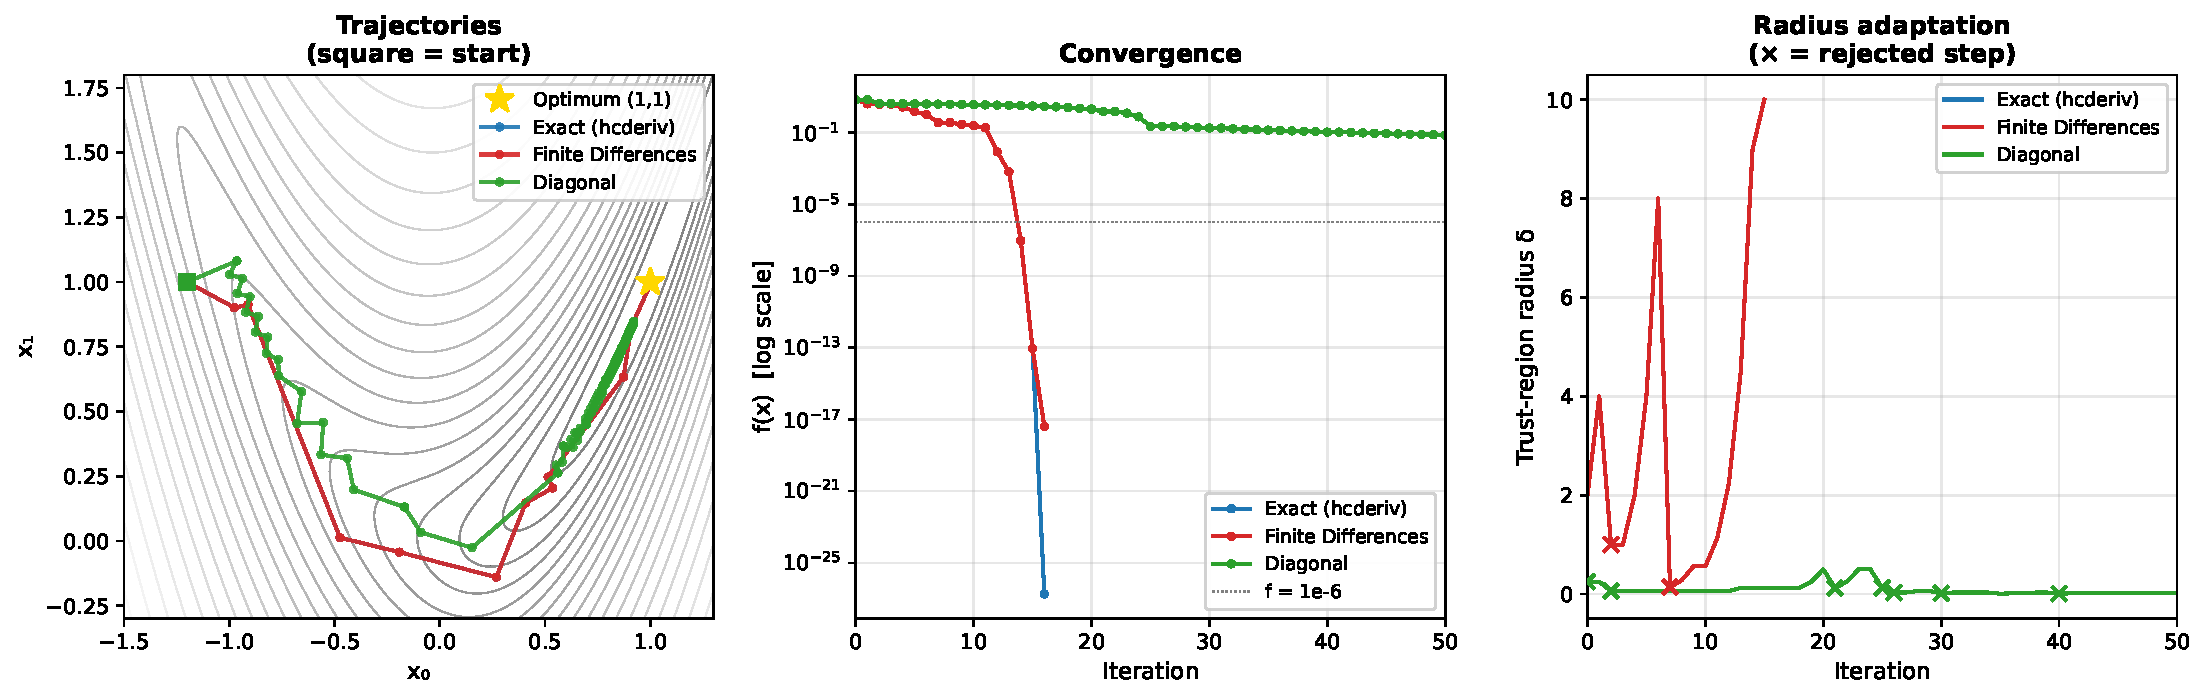
\includegraphics[width=\textwidth]{figures/trust_region_trajectories.pdf}
\caption{
  Trust-region optimization on the modified Rosenbrock function ($b=10$) from
  $(-1.2, 1.0)$. \textbf{Left:} optimizer trajectories on contour lines of
  $\log(1+f)$. Exact and FD solvers reach the optimum $(1,1)$ in 16 steps;
  the diagonal solver spirals in the valley without converging.
  \textbf{Center:} function value vs iteration (log scale). Exact and FD reach
  $f < 10^{-6}$ at iteration 14; diagonal stalls above $10^{-2}$.
  \textbf{Right:} trust-region radius adaptation. Exact and FD radii grow as
  Newton steps are accepted; diagonal radius oscillates (crosses = rejected steps).
}
\label{fig:trust_region}
\end{figure}

% ── 6. related work ───────────────────────────────────────────────────────────
\section{Related Work}

Second-order information is computationally expensive, and a substantial literature
addresses this cost through approximation. \citet{becker1989} proposed computing only
the diagonal of the Hessian at gradient-comparable cost by propagating squared
gradient terms forward through the network. \citet{elsayed2024} revisit and refine
this scheme as HesScale, demonstrating improvements over the original approximation
in both accuracy and applicability to reinforcement learning. These methods are
approximate by design: they trade the off-diagonal Hessian structure for scalability
to the parameter counts of deep networks ($d \sim 10^6$ to $10^9$).

The complex-step method \citep{lyness1967,squire1998} achieves machine-precision
first derivatives for scalar functions by perturbing the input into the complex plane.
It avoids the cancellation error that limits finite differences but does not extend to
second-order information without additional structure.

Algorithmic differentiation \citep{griewank2008} provides exact derivatives of
arbitrary order by augmenting the computational graph. Reverse-mode AD requires
$O(n)$ reverse passes for the full Hessian. JAX's \texttt{jax.hessian} is the
practical reference implementation and compiles to XLA. For fixed-point models,
unrolled AD differentiates through the iteration history rather than through the
fixed-point equation, producing iteration-depth-dependent curvature.

Hypercomplex perturbation occupies a complementary niche: exact full Hessians at
one-pass cost for moderate $n$, with IFT-correct derivatives for implicit models.
The tradeoff is the opposite of HesScale: full accuracy, bounded dimension.

% ── 7. limitations ────────────────────────────────────────────────────────────
\section{Limitations and Scope}

\paragraph{Scalar output.}
The algebra encodes the Hessian of $f:\mathbb{R}^n \to \mathbb{R}$. Vector-valued
functions require one hypercomplex pass per output dimension, equivalent in cost to
forward-mode AD applied per output.

\paragraph{Moderate $n$.}
The coefficient vector has length $1 + 3n + \frac{n(n-1)}{2}$, growing quadratically.
For $n = 100$ this is 5151 coefficients. Memory and compute scale as $O(n^2)$ per
multiply, making the method uncompetitive with diagonal approximations for deep
networks ($n \sim 10^{6+}$). The practical range is $n \sim 2$ to $100$.

\paragraph{Function expressibility.}
Functions must be implemented in hypercomplex arithmetic using the provided
\texttt{Hyper} methods (\texttt{.sin()}, \texttt{.exp()}, etc.), analogous to the
requirement in JAX that functions be written in \texttt{jnp}.

\paragraph{Not a replacement for diagonal approximations.}
HesScale and related methods address the deep-network regime where the full Hessian
is computationally inaccessible. hcderiv is complementary, not competitive.

\paragraph{No JIT compilation in the NumPy backend.}
A JAX backend (swapping \texttt{np} for \texttt{jnp}) would allow XLA compilation
and is a natural next step; the algebra is unchanged.

% ── 8. future work ────────────────────────────────────────────────────────────
\section{Future Work}

\paragraph{JAX/XLA backend.}
The algebra requires only array operations that map directly to \texttt{jnp}.
A \texttt{jit}-compiled backend would bring performance to parity with compiled AD
for moderate $n$, with an estimated additional 10--50$\times$ speedup.

\paragraph{Differentiable physics.}
Low-dimensional physical systems (pendulum, spring--mass, rigid body) lie in the
$n = 3$ to $30$ range and benefit from exact second-order sensitivity. The ridge
potential $U(x) = -\|f(x)\|^2$ studied in \citet{byte2026b} is one instance.

\paragraph{Implicit layers at scale.}
The IFT-correct Hessian demonstrated for $n = 3$ to $8$ generalizes to larger
implicit layers. Connecting hcderiv to deep equilibrium models \citep{bai2019}
or neural ODEs \citep{chen2018} would extend the method's reach to the implicit
differentiation literature.

\paragraph{Higher-order extensions.}
The two-unit algebra $(i_j, \varepsilon_j)$ recovers first and second derivatives.
A three-unit extension adds third-order terms, relevant to meta-learning and
hyperparameter sensitivity. The coefficient count grows as $O(n^3)$.

% ── 9. discussion ─────────────────────────────────────────────────────────────
\section{Discussion}

The results demonstrate that hypercomplex perturbation provides a practical and exact
mechanism for obtaining full Hessians in a single forward evaluation for scalar-valued
functions of moderate dimension. The method's strength lies in its algebraic
structure: by embedding first- and second-order Taylor coefficients into distinct
channels of a commuting infinitesimal algebra, the Hessian emerges as a byproduct of
ordinary function evaluation rather than a separate differentiation pass. This
reframes second-order computation not as an extension of algorithmic differentiation,
but as a representational choice about how inputs are encoded.

The empirical benchmarks highlight the consequences of this shift. For $n \lesssim
100$, the vectorized core achieves wall-clock performance comparable to gradient
evaluation while returning the full Hessian exactly. This places the method in a
region of the cost--accuracy landscape that is sparsely populated: exact curvature at
near-gradient cost. Diagonal approximations target the opposite regime, sacrificing
off-diagonal structure to scale to millions of parameters. The two approaches are
complementary, not competing.

The fixed-point experiments illustrate the conceptual advantage of the hypercomplex
formulation. For implicit models $z^* = f(z^*, \theta)$, the Hessian of the loss is
defined by the implicit function theorem, not by the unrolled iteration. Unrolled AD
produces iteration-dependent curvature. Hypercomplex perturbation perturbs the
converged fixed point directly and recovers the IFT-correct Hessian without
unrolling, a distinction that matters wherever curvature governs stability or
trust-region behavior.

Taken together, these results show that exact second-order information is not
inherently incompatible with efficiency. For low-dimensional physical systems, implicit
layers, parameter-sensitivity analysis, and small neural modules, the hypercomplex
approach provides a practical alternative to both finite differences and algorithmic
differentiation. The method does not aim to replace scalable approximations in deep
learning; rather, it fills the exact/moderate-$n$ corner of the design space that has
remained underserved.

% ── 10. conclusion ────────────────────────────────────────────────────────────
\section{Conclusion}

This work introduces a vectorized hypercomplex perturbation method that computes exact
full Hessians of scalar-valued functions in a single forward evaluation. By embedding
the first- and second-order Taylor structure into an augmented algebra, the method
achieves a cost profile comparable to gradient evaluation while returning full
curvature information without approximation. The implementation provides a NumPy-based
reference with complete reproducibility, a validated test suite, and empirical
benchmarks across dimensions and function classes.

The method's strengths are clearest for $n \sim 2$ to $100$, where exact curvature is
valuable and diagonal approximations offer limited benefit. The fixed-point
experiments demonstrate that the hypercomplex formulation naturally recovers the
IFT-correct Hessian without unrolling. The trust-region demo shows that exact
off-diagonal curvature qualitatively changes optimizer behavior: the diagonal baseline
stalls where exact and FD solvers converge in 16 steps.

Future work includes a JAX/XLA backend, differentiable-physics examples, extensions
to larger implicit layers, and higher-order generalizations. Together, these directions
point toward a broader ecosystem in which hypercomplex perturbation serves as a
practical primitive for exact second-order computation in scientific computing and
differentiable modeling.

% ── software availability ──────────────────────────────────────────────────────
\section*{Software Availability}

The software is available at \url{https://github.com/zetta55byte/hypercomplex}
under the MIT license. The v0.2.0 release is archived on Zenodo
\citep{byte2026c} with DOI \texttt{10.5281/zenodo.19389522} and is
installable via \texttt{pip install hcderiv}.

% ── ai usage disclosure ────────────────────────────────────────────────────────
\section*{License}

This paper is released under the Creative Commons Attribution 4.0 International
License (CC BY 4.0). The accompanying software is released under the MIT License.

\section*{AI Usage Disclosure}

This work was developed with assistance from Claude (Anthropic,
\texttt{claude-sonnet-4-6}, 2026). AI assistance was used for code generation
and refactoring, benchmark scripting, paper text drafting, and copy-editing.
All AI-assisted outputs were reviewed, validated, and edited by the author.
Core design decisions — algebraic structure, coefficient layout, vectorization
strategy, and benchmark methodology — were made by the author. The author takes
full responsibility for the accuracy and correctness of all materials.

% ── bibliography ──────────────────────────────────────────────────────────────
\bibliographystyle{plainnat}
\bibliography{references}

\end{document}
